
            \begin{figure}
                \centering
                \begin{tikzpicture}
                    \pgfplotsset{%
                        width=1\textwidth,
                        height=0.5\textheight
                    }
                    \begin{axis}[
                        xlabel={Start battery level},
                        ylabel={Average dynamic energy (watt)},
                    ]
                    
                        \addplot [mark=none, red, thick]  coordinates {
                        (40, 12.972930939299113)(45, 13.228403962568008)(50, 13.09891148723482)(55, 13.06811469290019)(60, 13.050950198212156)(65, 13.299765795558665)(70, 12.936703514502382)(75, 12.838390990716675)(80, 11.855165345802314)
                        };
                        \addlegendentry{Surface4Pro - IntelPowerGadget}
                        
                        \addplot [mark=none, red, dotted]  coordinates {
                        (40, 11.98720112075639)(45, 12.157245267251351)(50, 12.165010351934672)(55, 11.995975955070008)(60, 12.017428973531054)(65, 12.05434528264473)(70, 12.019644909181643)(75, 11.965369873795847)(80, 11.599367657326646)
                        };
                        \addlegendentry{Surface4Pro - HardwareMonitor}
                        
                        \addplot [mark=none, red, dashed]  coordinates {
                        (45, 8.059229605997768)(50, 8.049140167775192)(55, 8.045341589077072)(60, 8.035504316602333)(65, 8.02461608812454)(70, 8.011872957345993)(75, 8.024079801562358)(80, 7.945916093307767)
                        };
                        \addlegendentry{Surface4Pro - RAPL}
                        
                        \addplot [mark=none, blue, thick]  coordinates {
                        (40, 3.2391698817070744)(45, 3.5010080439499665)(50, 3.4825469531568407)(55, 3.579107066366934)(60, 3.4357354018088557)(65, 3.6311607501566323)(70, 4.125564412752033)(75, 3.4271095085441265)(80, 3.8854027626167476)
                        };
                        \addlegendentry{SurfaceBook - IntelPowerGadget}
                        
                        \addplot [mark=none, blue, dotted]  coordinates {
                        (40, 3.244953300492186)(45, 3.7991477755195504)(50, 3.6533842939401944)(55, 3.7268565054747023)(60, 3.640408305790674)(65, 3.4397384448945134)(70, 3.187387448505895)(75, 3.9510751856898083)(80, 3.066343131418361)
                        };
                        \addlegendentry{SurfaceBook - HardwareMonitor}
                        
                        \addplot [mark=none, blue, dashed]  coordinates {
                        (40, 4.926186425226801)(45, 4.9331872344630865)(50, 5.008365167699532)(55, 5.013996154142796)(60, 5.150838321245169)(65, 5.14928713251997)(70, 5.297331982928238)(75, 5.503383637558543)(80, 5.612919052972927)
                        };
                        \addlegendentry{SurfaceBook - RAPL}
                        
                    \end{axis}
                \end{tikzpicture} 
            \caption{A graph illustrating the energy consumption of Cores for test case BinaryTrees with regards to the battey level of the DUT} \label{fig:BinaryTrees_Cores}
            \end{figure}
            